\section{Experimental Setup}

\subsection*{Circuit components}
    \begin{enumerate}
        \item Transistor (CL100 or equivalent)
        \item Power supply
        \item 6 resistors of various specifications
        \item 3 Capacitors 
        \item Function Generator (~ 100-200 mV pp, sinusoidal for input signal)
        \item Oscilloscope
        \item Multimeters
        \item Connecting wires
        \item Breadboard
    \end{enumerate}

    \subsection*{Circuit Diagram}
    \begin{figure}[H]
        \centering
        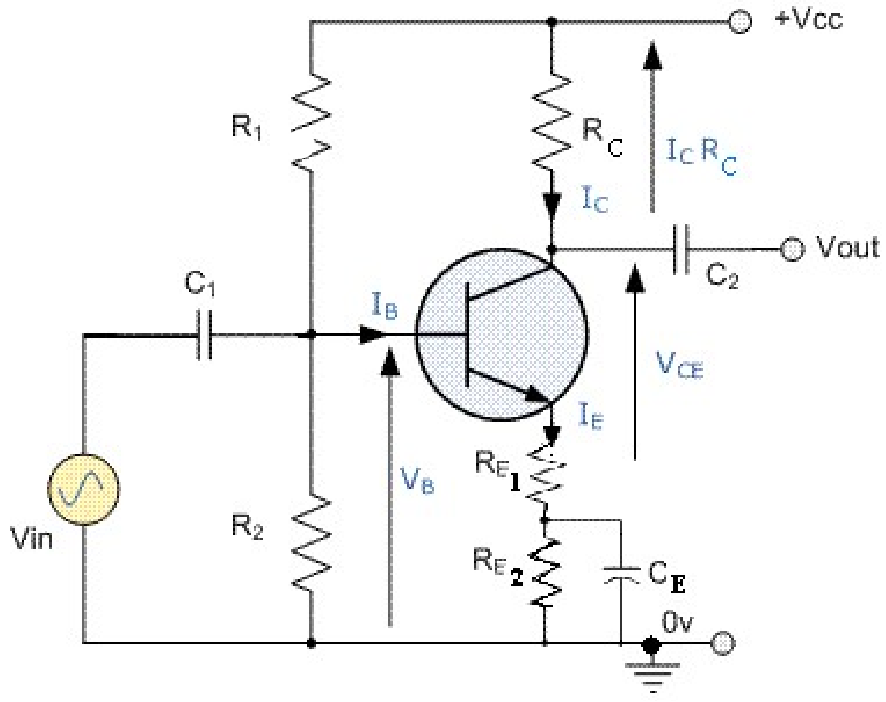
\includegraphics[width=1\columnwidth]{images/f1.png}
        \caption{Circuit diagram for the setup.}
        \label{fig:1}
    \end{figure}

\section{Data Analysis}
$\beta = $\\
$R_1=, R_2=$